% Created 2021-01-24 Sun 22:50
% Intended LaTeX compiler: pdflatex
\documentclass[11pt]{article}
\usepackage[utf8]{inputenc}
\usepackage[T1]{fontenc}
\usepackage{graphicx}
\usepackage{grffile}
\usepackage{longtable}
\usepackage{wrapfig}
\usepackage{rotating}
\usepackage[normalem]{ulem}
\usepackage{amsmath}
\usepackage{textcomp}
\usepackage{amssymb}
\usepackage{capt-of}
\usepackage{hyperref}
\usepackage{minted}
\hypersetup{colorlinks=true, linkcolor=black, filecolor=red, urlcolor=blue}
\usepackage[turkish]{babel}
\author{Eren Hatırnaz}
\date{11 Ağustos 2019}
\title{Yazılım Gündemi - 5\\\medskip
\large 5-11 Ağustos 2019}
\hypersetup{
 pdfauthor={Eren Hatırnaz},
 pdftitle={Yazılım Gündemi - 5},
 pdfkeywords={},
 pdfsubject={},
 pdfcreator={Emacs 27.1 (Org mode 9.3)},
 pdflang={Turkish}}
\begin{document}

\maketitle
\tableofcontents \clearpage\shorthandoff{=}

\begin{center}
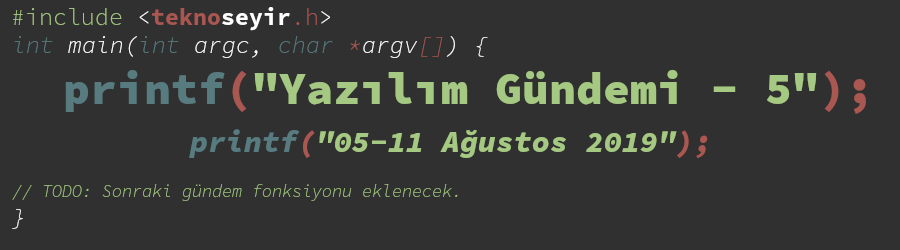
\includegraphics[width=.9\linewidth]{gorseller/yazilim-gundemi-banner.png}
\end{center}

\begin{center}
\href{../04/yazilim-gundemi-04.pdf}{< Önceki Gündem} | \textbf{5-11 Ağustos 2019} | \href{../06/yazilim-gundemi-06.pdf}{Sonraki Gündem >}

\href{https://teknoseyir.com/blog/yazilim-gundemi-5-05-11-agustos-2019}{TeknoSeyir'de Oku}
\end{center}

\section{GitHub Actions artık \href{https://github.blog/2019-08-08-github-actions-now-supports-ci-cd/}{CI/CD süreçlerini destekliyor}}
\label{sec:org5136d5a}
GitHub 8 Ağustos tarihinde kendi ofislerinde bir etkinlik gerçekleştirdi.
Etkinlik aynı zamanda canlı olarak \href{https://www.youtube.com/watch?v=E1OunoCyuhY}{YouTube üzerinden de yayınlandı}. Etkinliğin
asıl amacı yeni bir ürün/hizmet duyurmaktı fakat öncesinde GitHub'ın bu yıl
boyunca yaptığı şeylerin bir özetini geçtiler. Yayın başında hemen duyursalar
etkinlikler biterdi çünkü :). GitHub için 2019 yılı böyle geçiyormuş:
\begin{itemize}
\item Özel depoların (private repository) ücretsiz yapılması,
\item \href{https://github.com/features/package-registry}{Package Registry} hizmetinin duyurulması,
\item \href{https://github.com/dependabot}{Dependabot} projesi,
\item \href{https://github.com/sponsors}{Sponsors} özelliğinin duyurulması,
\item \href{https://github.blog/2019-06-17-github-acquires-pull-panda/}{Pull Panda'nın satın alınması},
\item \href{https://github.blog/2019-06-17-github-acquires-pull-panda/}{GitHub Desktop 2.0} sürümünün duyurulması,
\item 100'ün üzerinde üründe iyileştirmeler,
\item Bu hafta 40.000.000 geliştirici sayısına ulaşmışlar.
\end{itemize}

Etkinlikte söylememişler doğal olarak ama bir de Amerika'nın ambargo uyguladığı
ülkelerde yaşayan geliştiricilerin kodlarına el koyulması olayı var. \href{../03/yazilim-gundemi-03.pdf}{Yazılım
Gündemi - 3} yazısında detaylıca anlatmıştım.

Gelelim etkinlikte tanıtılan yeni özelliğe: GitHub Actions servisi artık
Continuous Integration ve Continuous Deployment süreçlerini destekliyor. Yani
artık bu süreçleri işletebilmek için travis-ci vb. gibi servisler yerine direkt
GitHub içindeki Actions servisi ile yapabilecekmişiz. Bazı özellikleri şu
şekilde:
\begin{itemize}
\item Matrix builds ile projenizin birden çok sürümünü aynı anda test etme,
\item Canlı log kayıtları,
\item Kod yazar gibi Action yazabilme
\end{itemize}

\url{gorseller/canli-loglar.gif}

Diğer özellikler için konu başlığına eklediğim bağlantıya tıklayabilirsiniz.
GitHub Actions henüz beta olduğu için bu özellikleri kullanabilmeniz için
Beta'ya kayıt yapmanız gerekiyor: \url{https://github.com/features/actions}.
\section{PHP topluluğundaki gruplar ve \href{https://wiki.php.net/pplusplus/faq}{P++ meselesi}}
\label{sec:org48578ec}
Bu hafta PHP Wiki'sinde yayınlanan sayfaya göre PHP topluluğunda iki grup
varmış. İlk grup, PHP'nin geçmişten gelen bazı özellikleri ve bakış açılarını
terk etmesi gerektiğini, daha kesin tiplendirilmiş bir dil olması gerektiğini;
diğer grup ise PHP'nin geçmişten gelen felsefesini ve özelliklerini korumak
gerektiğini savunuyor. Elbette böyle bir tartışmada "doğru" ya da "yanlış"
taraf yok. Herkesin kendine göre haklı nedenleri var.

P++'da tam olarak bu nedenden dolayı yapılmak istenen bir PHP lehçesi. Aklımıza
ilk geldiği gibi bir PHP 'fork'lanması, takımların ve projelerin ayrılması
durumu henüz söz konusu değil yani. P++ henüz bir kod ismi, kesin olarak bu
isim belirlenmedi ama bence bir kere bu şekilde duyurulduysa böyle devam
edecektir. P++, bildiğimiz PHP'ye göre çok daha sıkı kuralları olan ve farklı
özelliklere sahip bir lehçe olacak gibi duruyor. P++ dosyalarını işaretlemek
için şöyle bir yöntem önerilmiş:

\begin{minted}[breaklines=true,breakanywhere=true,frame=lines, linenos, label=PHP, labelposition=topline]{php}
<?p++?>
<?php echo "Merhaba TeknoSeyir!" ?>
\end{minted}

PHP mail grubunda ve \href{https://www.reddit.com/r/programming/comments/cohb0r/p/}{Reddit} gibi platformlarda tartışmalar devam ediyor.
Bakalım ne olacak\ldots{}
\section{Visual Studio Code \href{https://code.visualstudio.com/updates/v1\_37}{Temmuz 2019 güncellemesi yayınlandı}}
\label{sec:orgb45ba88}
\begin{center}

\includegraphics[width=.9\linewidth]{gorseller/vscode-temmuz2019.png}
\end{center}
\section{Diğer Haberler}
\label{sec:org779b2aa}
\begin{itemize}
\item PHP 7.4.0 \href{https://www.php.net/archive/2019.php\#2019-08-08-1}{Beta 2 yayınlandı}, \href{https://github.com/php/php-src/blob/php-7.4.0beta2/NEWS}{değişiklik notları}, \href{https://downloads.php.net/\~derick/}{indirme bağlantıları}.
\item PHP-FIG (Framework Interop Group) topluluğu \href{https://github.com/php-fig/fig-standards/blob/master/accepted/PSR-12-extended-coding-style-guide.md}{PSR-12 (Genişletilmiş Kod Stili
Rehberi) standardını kabul etti}.
\item Alman Havacılık Merkezi (German Aerospace Center - DLR), CosmoScoutVR isimli
modüler sanal evren projesini \href{https://github.com/cosmoscout/cosmoscout-vr}{açık kaynak olarak yayınladı}.
\item Microsoft, Azure Security Lab hizmetini \href{https://venturebeat.com/2019/08/05/microsoft-launches-azure-security-lab-doubles-top-bug-bounty-to-40000/}{duyurdu ve açık bulanlara verilen
ödülü arttırdı}.
\item ASP.NET Community Standup yeni bölümü yayınlandı: \href{https://www.youtube.com/watch?v=t5sBSOydYxI}{ASP.NET Core A to Z eBook
with Shahed Chowdhuri}.
\item NVIDIA açık kaynak sürücülere destek için \href{https://www.phoronix.com/scan.php?page=news\_item\&px=NVIDIA-Open-GPU-Docs}{donanımsal dökümanlar paylaşmaya
başladı}.
\item Gleam programlama dilinin \href{https://lpil.uk/blog/gleam-v0.3-released/}{v0.3 sürümü yayınlandı}, \href{https://github.com/lpil/gleam}{GitHub Deposu}.
\item Git deponuzun tarihçesini düzenleme olanacağı sunan araç \href{https://mystor.github.io/git-revise.html}{açık kaynak olarak
yayınlandı}: \href{https://github.com/mystor/git-revise}{Git-Revise}.
\item BlazingSQL isimli donanım hızlandırmalı SQL motoru \href{https://blog.blazingdb.com/blazingsql-is-now-open-source-b859d342ec20}{açık kaynak olarak
yayınlandı}, \href{https://github.com/blazingdb/pyBlazing/}{GitHub Deposu}.
\item Bulut uygulamaları için yayınlama (deploy) işlerini kolaylaştırma iddiası
taşıyan \href{https://ic.dev/}{IC} isimli proje \href{https://medium.com/icdotdev/introducing-ic-b3eabf8bf120}{açık kaynak olarak yayınlandı}, \href{https://github.com/icdotdev/cli}{GitHub Deposu}.
\item Android uygulama geliştirme için mail gönderme kütüphanesi açık kaynak
olarak yayınlandı: \href{https://github.com/nedimf/maildroid}{maildroid}.
\item Terminal çıktılarında tıklanabilir linkler oluşturmaya yarayan kütüphane
açık kaynak olarak yayınlandı: \href{https://github.com/piotrmurach/tty-link}{tty-link}.
\item Jekyll \href{https://jekyllrb.com/news/2019/08/04/jekyll-4-0-0-pre-beta1-released/}{4.0.0.pre.beta1 sürümü yayınlandı}.
\item JavaScript için yeni bir para birimi kütüphanesi yayınlandı: \href{https://github.com/xxczaki/cashify}{Cashify}.
\item Vue-Router \href{https://github.com/vuejs/vue-router/releases/tag/v3.1.0}{v3.1.0 sürümü çıktı}.
\item Kotlin ile yazılmış shell Kash, \href{https://github.com/cbeust/kash/releases/tag/v1.14}{v1.14 sürümünü çıkardı}.
\item VectorClass kütüphanesinde \href{https://www.agner.org/optimize/blog/read.php?i=1013}{büyük değişiklikler var}.
\item Lazarus, \href{https://www.getlazarus.org/release/}{2.0.4 sürümünü duyurdu}, \href{https://wiki.lazarus.freepascal.org/Lazarus\_2.0.0\_release\_notes}{Değişiklik notları}.
\item OpenAPI Generator \href{https://github.com/OpenAPITools/openapi-generator/releases/tag/v4.1.0}{4.1.0 sürümü çıktı}.
\end{itemize}
\section{Lisans}
\label{sec:orgec730bf}
\begin{center}
\begin{center}

\includegraphics[height=1.5cm]{../../../img/CC_BY-NC-SA_4.0.png}
\end{center}

\href{yazilim-gundemi-05.pdf}{Yazılım Gündemi - 5} yazısı \href{https://erenhatirnaz.github.io}{Eren Hatırnaz} tarafından \href{http://creativecommons.org/licenses/by-nc-sa/4.0/}{Creative Commons
Atıf-GayriTicari-AynıLisanslaPaylaş 4.0 Uluslararası Lisansı} (CC BY-NC-SA 4.0)
ile lisanslanmıştır.
\end{center}
\end{document}
